\newpage
\subsection{Transformations}\label{subsec:Transformations}
Les transformations sont une des spécificités les plus utiles et uniques du $Ray\ Marching$. En effet, elles sont extrêmement peu coûteuses en ressources, et permettent de créer des formes uniques.
\\Pour toutes transformations il suffit, lorsqu'on veut obtenir la distance entre un point $P$ de l'espace et un objet transformé, de prendre la distance entre la \textbf{transformation inverse} du point $P$ et l'objet non transformé.
\begin{align*}
    SDF\_Objet\_Tranforme(P)=SDF\_Objet(Transformation\_Inverse(P))
\end{align*}
Nous allons maintenant voir quelques exemples.

\subsubsection{Translation}
Pour obtenir une translation de vecteur $translation$ d'un objet, on peut utiliser le code suivant :
\begin{lstlisting}[language=GLSL]
SDL_Objet(p-translation);
\end{lstlisting}

\subsubsection{Rotation autour des axes XYZ}
Pour une rotation autour des axes X, Y et Z, d'angles respectivement $alpha$, $beta$ et $gamma$ d'un objet, on utilise le code suivant:
\begin{lstlisting}[language=GLSL]
SDL_Objet(Rotation(p,-alpha,-beta,-gamma))
\end{lstlisting}
Avec $Rotation$ une application linéaire dont la matrice dans la base cannonique est donnée ici : 
\begin{align*}
    R(x,y,z)
    =& R_{ex}(x)R_{ey}(y)R_{ez}(z) \\
    = &
    \begin{bmatrix}
    cos(x) & -sin(x) & 0 \\
    sin(x) & cos(x) & 0 \\
    0 & 0 & 1 
    \end{bmatrix}
    \begin{bmatrix}
    cos(y) & 0 & sin(y) \\
    0 & 1 & 0 \\
    -sin(y) & 0 & cos(y) 
    \end{bmatrix}
    \begin{bmatrix}
    1 & 0 & 0 \\
    0 & cos(z) & -sin(z) \\
    0 & sin(z) & cos(z) 
    \end{bmatrix}\\
    = & \begin{bmatrix}
    cos(y)cos(z) & sin(x)sin(y)cos(z) & cos(x)sin(y)cos(z)+sin(x)sin(z) \\
    cos(y)sin(z) & sin(x)sin(y)sin(z)+cos(x)cos(z) & cos(x)sin(y)sin(z)-sin(x)cos(z) \\
    -sin(y) & sin(x)cos(y) & cos(x)cos(y)
    \end{bmatrix} \\
\end{align*}

\subsubsection{Duplication des volumes}
Il est egalement possible d'appliquer des transformations plus complexes, permettant par exemple la duplication d'objets. Pour dupliquer un nombre infini de fois un volume, il suffit d'appliquer un modulo (reste de la division entière) sur la position de l'objet.
\\Le code pour dupliquer un objet à l'infini sur l'axe Ox, toutes les $N$ unités, est celui-ci:
\begin{lstlisting}[language=GLSL]
SDF_Objet( vec3( mod(p.x - N/2, N) + N/2, p.y, p.z))
\end{lstlisting}
\textbf{Remarque:} $vec3$ est un constructeur de vecteur 3D
\begin{figure}[h]
    \centering
    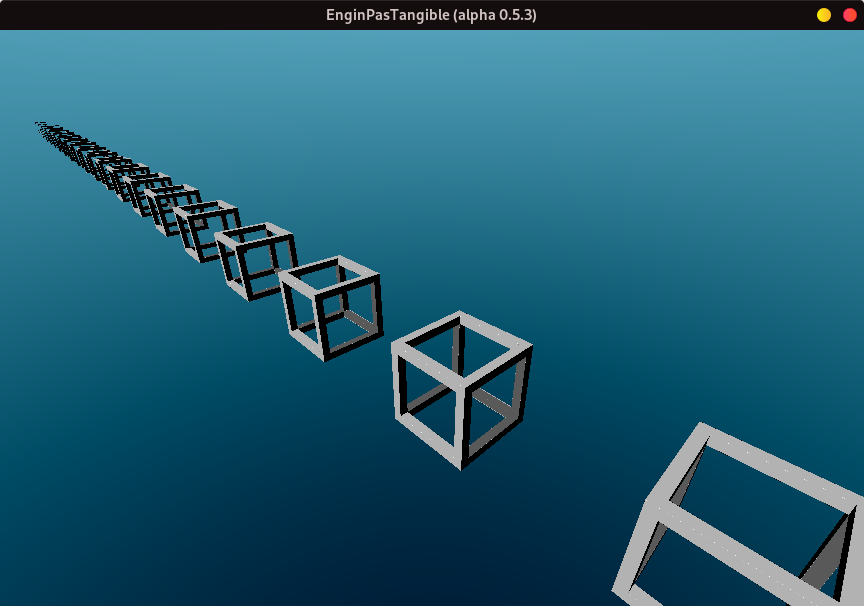
\includegraphics[width=6cm]{images/screens/infinite.png}
    \caption{Duplication d'un objet à l'infini}
    \label{fig:infinite}
\end{figure}

\subsubsection{Symétrie}
Il est egalement possible de faire des symétries par rapport à un plan de normale $N$ et de décalage $offset$. Le code est le suivant:
\begin{lstlisting}[language=GLSL]
SDF_Objet(symetrie(p,-normale,-offset));
\end{lstlisting}
Avec le code de $symetrie$ :
\begin{lstlisting}[language=GLSL]
vec3 symetrie(vec3 position, vec3 normale,float offset){
    float d=dot(position,normale) + offset;
    if (d>0) return position;
    else return position-2.0*d*normale;
}
\end{lstlisting}
Avec $dot$ le produit scalaire.
\\\textbf{Remarque:} Cette symétrie ne fonctionne que dans un seul sens. C'est à dire que l'un des côtés du plan "disparaît" pour laisser place au symétrique de l'autre côté du plan.